\documentclass[12pt]{article}
\usepackage{amsmath}
\usepackage{amsfonts}
\usepackage[utf8]{inputenc}
\usepackage[T1]{fontenc}
\usepackage{graphicx}
\begin{document}

\topskip0pt
\begin{center}
	\vspace*{1cm}
	
	\textbf{Game Design Document}
	
	\vspace*{4cm}
	\begin{itemize}
		\item \textbf{Game Title}: Y.O.L.T. (You Only Live Twice)
		\item \textbf{Team Name}: Seaside Games
		\item \textbf{Team Members}:
		\begin{itemize}
			\item Nunzio Arcifa (921559)
			\item Matteo Dell'Oro (910238)
			\item Alfio Giuliano Faro (908958)
			\item Chen Qixuan (10592030 - Polimi)
			\item Maura Saccà (894850)
		\end{itemize}
		\item \textbf{Academic Year}: 2017/2018
	\end{itemize}
	
\end{center}

\newpage

\tableofcontents

\newpage

\section{Design History}

\begin{itemize}
	\item \textbf{v1.0} - Document Created
	\item \textbf{v1.1} - Formatting changes
	\item \textbf{v1.2} - Changed Music and Sound FX to only Sound FX in section 9
\end{itemize}

\newpage

\section{Vision Statement}

\subsection{Game Logline}

Fight to the last man, but don't be afraid to take one for the team, as dying is just the beginning.

\subsection{Gameplay Synopsis}

Each player has to move around the map and shoot the enemies which come in waves. Once a player dies, he becomes a “ghost”, in this state, he can move around the map and collect lùth, resource obtainable from defeating dead enemies, used to link their movement to the one of an ally player who is still alive. In this linking state, he can choose among 3 different classes: Assassin, with massive damage potential, Tank, with shielding and crowd control capabilities, and Support, with healing and debuff abilities. While the player is in this state, he runs out of lùth over time: when this resource is over, he returns to be a “ghost”. When every player has died the game is over; the player although will win the match once the final boss is defeated.

\newpage

\section{Audience, Platform and Marketing}

\subsection{Target Audience}

This game is focused for players who wants to cooperate with other players act to reach a common goal. The minimum recommended age is 16, cause darker themes are present in game. There is no indicated geographic location.

\subsection{Platform}

PC, PS4, XBOX1. No mobile platforms as the game mechanics make the gameplay too difficult on a handheld device. Console were considered as the “plug-and-play” style of the game, with fast matches, is suitable to be played on those.

\subsection{Top Performers}

\begin{itemize}
	\item Call of Duty: Zombie Mode
	\item Gauntlet
	\item Magika
	\item Dead Nation
	\item Gears of War: Horde Mode
	\item Enter the Gungeon
\end{itemize}

\subsection{Feature Comparison}

The game camera is exactly like games such as Gauntlet, Magika, Dead Nation.

In Call Of Duty: Zombie Mode a player uses money earned by killing zombies to expand the map. In Y.O.L.T we use the same method with a little difference consisting in the requirement of having every player contribute with the same amount of currency, earned by killing enemies, to open buildings and expand the map. The spawn technique for enemies is the same, once the map gets bigger there will be several spawn point to keep under control.

In Gauntlet the players group is formed by 4 people, which name can be chosen as in our game; the difference is that in Gauntlet there are monster hordes that are sometimes visible on a not accessible side of the map, which will eventually swarm you after some time. On the other hand in Y.O.L.T. monster hordes will come from points in the map that are not visible. Gauntlet have you facing enemies one after the others in various rooms, while Y.O.L.T. has waves with fixed amount of enemies, regardless of how much the map has been expanded. If you choose to fight every enemy in the starting area of the map it will be hard not to be overcome in such limited space. 

In Heroes of the Storm, the hero Cho’Gall is controlled by two players at the same time: one is Cho, mainly controlling the movement and the second uses Gall, a powerful spell caster. In our game once the player dies he’ll be able to act like Gall does, connecting themselves to an alive hero using spells while not able to control the movement (which is bound by the alive player below).

In the cooperative mode of Enter The Gungeon, when one of two player dies he can’t shoot anymore but he can still move around the map and doing some disrupting action, like destroying the bullet which points to the ally who is still alive. In our game, when a player dies, their game is not over but aside from disrupting action he can also enhance alive players with shields, healing and even damage.

\newpage

\section{Gameplay}

\subsection{Overview}

Y.O.L.T is a shooter game with isometric camera, in a 3D environment. The player commands a character which shoots and kills various enemies. When a character dies, the player will become a “ghost” to examine the area around the team, to advice the other players about the danger, and after collecting enough lùth, he will become a character’s add-on, linked to an alive player for a limited time. When the player runs out of lùth, he turns back the “ghost” state. When the resource is filled up again, the player can attach themselves again. If one of the alive players uses the Resurrection item on them, that player can come back to life.

\subsection{Gameplay Description}

At the beginning of the game your character is the same as the other one, only their colours changes to distinguish with each other. The player’s character can buy a little robot that shoot enemies and can eventually be used as a static machine gun controlled by AI. Using your character, your objective is to shoot against the enemy to kill them; slaying enemies provides you with currency, used to unlock more powerful weapons, skills and tools. The main objective of course, is to survive as long as possible.

Every character is able to move around the battle zone, cooperate with other players and reach team’s objectives. When their character dies, he will continue to play as a “ghost”: in this state the player is able to move around the area and warn their teammates about the dangers, enemies and powerups while collect lùth which will be used to link their movement with one of the teammates who is still alive.

Once attached to a fellow player, you have to decide among 3 different classes: Assassin, that unlocks damage and attack skills, Tank, which gives you defense capabilities and the possibility of taunting enemies, and Support, which can heal the alive players and debuff spells. If the attached player lùth ends, the player comes back into “ghost” form and have to collect that resource again to fuse another time.

Kill after kill, you achieve some currency, spendable to Yaff’s shop in exchange of items and weapons; that currency can also be used to buy access to other areas of the level, to expand the map. Enemies spawn in waves, with a boss wave coming once every 3 normal ones are cleared; the boss waves require exceptional coordination with the team.

\subsection{Controls}

\subsubsection{Interfaces}

\textbf{Outside Game Interfaces}
\begin{enumerate}
	\item When the user launch the game, he is asked to insert their character’s name.
	\item The home includes a Room List and buttons such as “Create a Room”, “Join a Room” and “Options”.
\end{enumerate}

\textbf{Inside Game Interfaces}
\begin{enumerate}
	\setcounter{enumi}{2}
	\item The Main In-Game Interface which includes health bars, used weapon, available skills and currency amount.
	\item The Merchant UI lets the player buy upgrades and special items.
	\item The Choosing Class UI lets the player choose their class, clicking on one of three differents buttons: “Support”, “Tank” and “Assassin”.
	\item After the Choosing Class UI the player is then asked to choose the alive companion he wants to be attached with.
	\item When a player uses the special object to resurrect another player, the Resurrect UI will let him choose which player he wants to bring back to life.
\end{enumerate}

\subsubsection{Rules}

The game has players who shoot with weapons at enemies coming in waves. After all the enemies of a wave are killed, players will have a small amount of time to prepare themselves for the next wave. A player can buy upgrades and special items both in the wave time and in the pause time between waves. The player movements are limited by the terrain and walls. The NPCs can move in the map but they can be blocked by different features.

Every player can buy allied Pets that shoot enemies with line-of-sight techniques: they follow players and can eventually be placed on the ground in order to improve their firerate. When a player, or their Pets, kill an enemy NPC they will get a fixed amount of currency.

The game map is divided between different areas. The player can enlarge the map using the currency he get from the kills. The only way to enlarge the map and, consequently, have more mobility and resources to kill all enemies, is that each player will have to contribute with the same (fixed) amount of currency needed to unlock that new area. In case one of the players doesn’t reach the minimum amount of currency, or simply doesn’t pay that, all the players will be restricted to the current area, where more difficult waves can be problematic.

Once a player dies he will become a “ghost” and, once with enough lùth, he can link his movement to the one of an ally player who is still alive, by becoming a sort of addon of that character. When a player become a “ghost” they are useful to the team in terms of examining the area and giving advice the players on enemies movements and locations.

When an enemy dies he will drop lùth, that fills up a bar of the player. When the bar is fully restored they will have the possibility to link themselves to an alive partner choosing among 3 classes: Assassin, with massive damage potential, Tank, with shielding and crowd control capabilities, and Support, with healing and debuff abilities.

\subsubsection{Scoring/Winning Conditions}

The game time is divided by waves of enemies. Each wave has a fixed number of enemies to kill. After all the enemies are killed there will be a little pause, before the next wave will start. This procedure will happen until all the players are dead or until the players manage to arrive at the final boss wave. If they can defeat the boss they can decide to end the game or to continue until all the players are dead, introducing an “endless” type of gameplay.

The leaderboard rankings are sorted by waves cleared; between parties with the same number of waves cleared, a high score is taken into account which is calculated with an algorithm using time spent in the game and currency saved. 

\subsection{Modes and other Features}

The game main mode is multiplayer cooperative survival where 2 to 4 players have to split their focus between attacking the enemies and helping their fellows in order to overcome all the challenges. The game will last 12 waves, with the a boss coming every 3 waves and the final boss coming at the last one. Once the fubak boss is defeated the game is won, but players can continue playing to see how far they last.

Another, secondary game mode is the multiplayer competitive arena, still in development and not currently in the game.

An additional mode is the tutorial one, where players can learn how to play the survival game mode in a safe and controlled environment.

\subsection{Levels}

The survival game mode features at the moment only one level, with more to be added in future patches. The players start in an enclosed area with few entrances, and eventually can unlock more areas with a fixed price in order to create more space and throttle enemies in bottlenecks, to aid the clearing. The level has both natural and artificial props and walls used to find cover from enemy bullets.

\subsection{Flowchart}

\begin{center}
	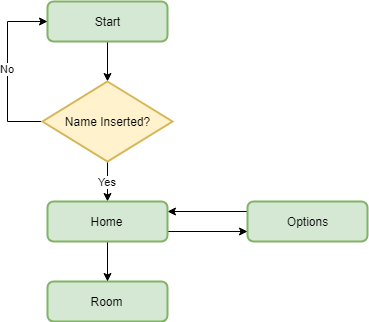
\includegraphics[width=0.5\textwidth]{Diagramma1}
	\newline\newline\newline
	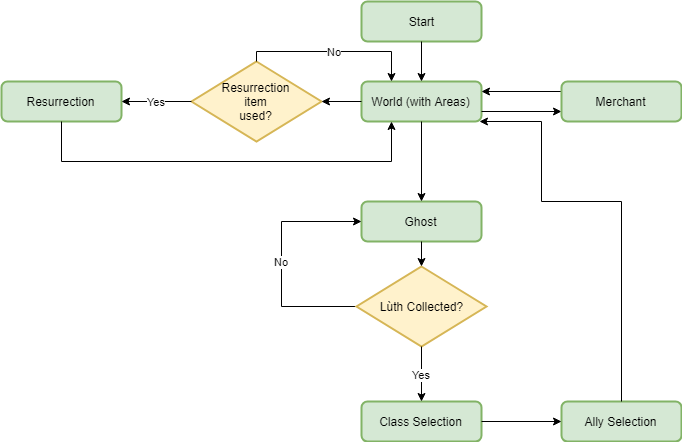
\includegraphics[width=0.8\textwidth]{Diagramma2}
\end{center}

\newpage

\section{Game Characters}

\subsection{Player Characters}

\begin{itemize}
	\item \textbf{Soldiers} - Players’ initial characters are sent into the World Between to bring back the order and the proper division between the dead and the alive. Every player’s character has the same abilities as the others, and only after death there is a diversification in terms of choosable classes.
	\item \textbf{Ghosts} - After a player dies, they will become a “ghost”, which can explore the map and give advice to their group about the closest dangers. They collect lùth, which is used to fuse with a teammate until it uses up. When it has achieved a certain quantity of it, you have to choose among 3 classes.
	\item \textbf{Assassin} - This class unlocks new attacks and skills, while improving attack speed of the attached onto character.
	\item \textbf{Tank} - This class unlocks shielding and crowd controlling capabilities, while augmenting the attached character’s health points.
	\item \textbf{Support} - This class unlocks healing and debuffing spells, while improving the movement speed of the attached onto character.
\end{itemize}

\subsection{Non Player Characters}

\begin{itemize}
	\item \textbf{Yaff} - It’s a gnome, the only inhabitant of the World Between and nobody knows how he ended up there. This NPC sells every sort of item useful to properly fight the battle; defeating enemies gives currency spendable at his shop, where you can buy weapons, equipment and other items.
	\item \textbf{Pet} - Purchasable robot that follows its owner. He shoots enemies while alongside the player or can be placed in the fighting area, locking it in a static state and improving its fire rate.
	\item \textbf{Melee Dead} - The basic enemy which can only hit the players from short range with melee attack.
	\item \textbf{Frenzied Dead} - Another melee enemy with faster attack speed/movement.
	\item \textbf{Ranged Dead} - Enemy hitting from the distance, slower and less resistant, but with stronger shots.
	\item \textbf{Cleric Dead} - Enemy regenerating the health points of the nearby dead, more resistant than the normal enemies. Enemies tend to gather around it, in order to protect him and receive its heals.
	\item \textbf{Gatekeeper} - Every 3 waves a gatekeeper spawns as a boss. Bosses are different between each other, and the 4th boss is the final one and much stronger than the previous.
\end{itemize}

\newpage

\section{Story}

\subsection{Synopsis}

The order between the Life World and the Dead World is broken. For thousands of years Gatekeepers had always protected the two Portals that are built in the World Between. These Portals managed to keep the two worlds separated, as they only open when a person of the Life World dies, to make him pass through.

In the Life World some explorers found and used an ancient artifact without knowing its true power: it can resurrect the dead. This angered the Gatekeepers, as they are the only ones who can supervise the passage between life and death. So they decided to abandon their duties in order to punish the living, leaving the Portals unprotected and, doing so, destroying the balance between those two dimensions. Here is where the story of four brave men begins: they were sent in the World Between where, with the help of the gnome Yaff, they need to fight in order to avoid the return of the dead on the living realm and restore the order of the worlds. 

\subsection{Backstory}

In an uncertain future people live normally their life. They come, live and die. The, so called, Life World is the realm where they prosper and live a full life, focused on building families and improve their technologies. When a person dies their body disappear and finishes in the Dead World. In contrast to the Life World, this realm is the opposite of peace and prosperity. The more people stay in that world, the more they become apathetic and even hostile. All the sins they made when they were alive come to their memory and this burden makes them wary and coy. The desire of leaving this land full of sinners grow inside them until the point that is the only thing remaining in their mind. But they will never leave the Dead World, it is their destiny.

The only thing that links these two Worlds is the World Between. This realm is protected by the Gatekeepers, which job is to supervise the two Portals connecting these realms, a duty that they have been doing for thousand of years. 
The only inhabitant of the World Between is Yaff, a mysterious gnome that tries to survive in this uncomfortable place. No one knows why he is there, where he has been living alone for years.

\newpage

\section{The Game World}

The game world is a fictional one in Y.O.L.T. There are no key locations, everywhere is just the World Between, where the dead get in touch with the living through the portals, and the gatekeepers roam around wrecking havoc. There is no weather conditions, outside of a constant and permanent fog that surrounds the whole scene; also, night, day and time in general have no meaning in such a world.

The scale of the world is technically infinite, but limited in-game in order to implement proper gameplay. The physics are close to the ones of the real world, even though some elements and properties like gravity can be a little different.

Not belonging to the World Between, soldiers (player characters) entered the world with the aim of trying to restore the balance of the life cycles. As foreign beings, their presence is easy to spot and their bodies are not fully accustomized to the world features yet.

\newpage

\section{Media List}

\begin{itemize}
	\item \textbf{Interface Assets} - HP Counter (both player and eventual pet), Weapon Used Icon, Wave Counter (with Mobs missing to next wave), Ability Cooldowns, Activatable Items Icons.
	\item \textbf{Environments} - Level with the areas
	\item \textbf{Characters} - Assassin, Tank, Support, Ghost, Pets, Yaff, Mobs, Gatekeepers, Final Gatekeepers
	\item \textbf{Animations}
	\begin{itemize}
		\item \underline{PCs} - Running, Shooting, Spell Usage, Death
		\item \underline{Pets} - Running, Shooting, Death
		\item \underline{Mobs} - Running, Shooting, Death
		\item \underline{Gatekeepers} - Running, Shooting, Spell Usage, Death
	\end{itemize}
	\item \textbf{Sound FX} - Level Music, Players SFX (Footsteps, Shot, Spell Usage, Death, Currency Increase, Buy), Pets SFX, Enemies SFX (Footsteps, Shot, Death), Gatekeepers SFX, Players/Gatekeepers/Yaff Voice Lines, Environment Sounds, Resurrection, Enlarge the Map.
\end{itemize}

\newpage

\section{Background Music}

The music follows the series of waves and pausing time of the game. So there are battle tracks, animated and fast, that increase intensity when the players overcome waves until the final boss, and quiet and slow tracks between the waves.

Music will change considering the class picked, in that short amount of time.

Every three waves, the music will change to emphasize the fact that we are fighting the bosses.

\begin{itemize}
	\item \textbf{Reference Waves}
	\begin{itemize}
		\item Don’t be afraid (from Final Fantasy VIII)
		\item Battleship Titan (from Xenoblade Chronicles 2)
		\item Night of Fate (from Kingdom Hearts)
	\end{itemize}
	\item \textbf{Reference Pausing Time}
	\begin{itemize}
		\item Mako Reactor (from Final Fantasy VII)
		\item Shrine (from The Legend of Zelda - Breath of the Wild)
	\end{itemize}
\end{itemize}

% \newpage

% \section{Prototype Features List}



\end{document}